\section{Pre-procesamiento}
Para empezar con el pre-procesamiento, vamos a transformar a factores todas las
variables que se especifican como categóricas en la competición de kaggle.
Además, pasaremos las variables \textit{TransactionAmt} (cantidad de dinero) y
\textit{TransactionDT} (delta de tiempo) a intervalos y eliminaremos el ID de la
transacción. La clase objetivo \textit{isFraud} se cambia a valores con un
significado más claro (de 1 y 0 a \textit{Yes} y \textit{No}).

\begin{lstlisting}
data_discretized <- 
    train_dataset %>%
    mutate(isFraud = as.factor(ifelse(isFraud == 1, "Yes", "No"))) %>%
    mutate_at(c("ProductCD", "P_emaildomain", "R_emaildomain", "DeviceType", "DeviceInfo"), factor) %>%
    mutate_at(vars(starts_with("addr")), factor) %>%
    mutate_at(vars(starts_with("card")), factor) %>%
    mutate_at(vars(starts_with("M")), factor) %>%
    mutate_at(vars(matches("id_(1[2-9]|2[0-9]|3[0-8])")), factor) %>%
    mutate(
      TransactionAmt = cut_number(TransactionAmt, n = 10),
      TransactionDT = cut_number(TransactionDT, n = 10)
      ) %>%
    select(-TransactionID)
\end{lstlisting}

A partir de la información aportada por \lstinline{df_status()}, podemos
eliminar directamente las variables con gran porcentaje de valores NA y
dispersión muy alta o muy baja. En mi caso, elimino todas aquellas variables
con más de un 50\% de valores vacíos, más de un 80\% de dispersión y las
variables numéricas con menos de un 1\% de dispersión.

\begin{lstlisting}
library(funModeling)

status <- df_status(data_discretized)

na_cols <- 
  status %>%
  filter(p_na > 50) %>%
  select(variable)

high_dif_cols <- 
  status %>%
  filter(unique > 0.8 * nrow(data_discretized)) %>%
  select(variable)

low_dif_cols <-
  status %>%
  filter(type == "numeric" & unique < 0.01 * nrow(data_discretized)) %>%
  select(variable)

data_reduced <-
  data_discretized %>%
  select(-one_of(
    bind_rows(list(na_cols, high_dif_cols, low_dif_cols))$variable
    ))
\end{lstlisting}

Una vez eliminadas estas variables, todavía quedan en el conjunto de datos
valores vacíos, los cuáles tenemos que reemplazar. Si se trata de variables
numéricas, sustituiremos con el valor medio de la variable usando la función
\lstinline{na.aggregate} del paquete \textit{zoo}, mientras que si son
categóricas, usaremos una nueva categoría \textit{Unknown}.

\begin{lstlisting}
library(zoo)

data_replaced <-
  data_reduced %>%
  mutate_if(is.numeric, na.aggregate) %>%
  mutate_if(is.factor, fct_explicit_na, na_level = "Unknown")
\end{lstlisting}

Calculando la matriz de correlación y usando la función
\lstinline{findCorrelation()} del paquete \textit{caret}, podemos obtener una
lista de variables que se pueden eliminar del conjunto de datos debido a que
poseen alta correlación con otras variables. En mi caso, he buscado las que
tengan una correlación superior a 0,8.

\begin{lstlisting}
library(caret)
library(reshape2)

corr_matrix <-
    data_replaced %>%
    select_if(is.numeric) %>%
    cor(.)

data_final <-
    data_replaced %>%
    select(-one_of(findCorrelation(corr_matrix, cutoff = 0.8, names = TRUE)))
\end{lstlisting}

Después de todo este tratamiento, nos quedan todavía 54 variables. Vamos a
reducir aún más este número usando una técnica especializada de extracción de
variables conocida como \textit{Boruta}. Esta función seleccionará y rechazará
variables en base a su importancia calculada. En mi caso, la función
seleccionaba todas las variables, por lo que decidí quedarme con las 10 que más
importancia media tenían.

\begin{lstlisting}
library(Boruta)

boruta_output <- Boruta(isFraud ~ ., data = data_final, doTrace = 2)

imp_cols <-
  attStats(boruta_output) %>%
  rownames_to_column(var = "variable") %>%
  top_n(10, meanImp) %>%
  select(variable)

data_boruta <-
  data_final %>%
  select(isFraud, one_of(imp_cols$variable))
\end{lstlisting}

Ya tenemos nuestro conjunto de datos final con tan solo 10 variables, tamaño que
podemos gestionar con facilidad. Sin embargo, seguimos teniendo el problema del
desbalanceo de la clase objetivo que vimos en la exploración de los datos. Para
solucionar esto, vamos a aplicar técnicas de generación sintética de datos
(combinando \textit{undersampling} y \textit{oversampling}). En concreto,
usaremos ROSE y SMOTE, obteniendo dos conjuntos de datos balanceados diferentes
sobre los que entrenaremos los mismos clasificadores para comprobar el
impacto de ambas técnicas en la calidad de las predicciones. En las figuras
\ref{fig:class-rose-barplot} y \ref{fig:class-smote-barplot} se puede ver el
nuevo reparto de registros tras aplicar ROSE y SMOTE, respectivamente.

\begin{lstlisting}
library(ROSE)
library(DMwR)

data_balanced_rose <- ROSE(isFraud ~ ., data = data_boruta, seed = 1)$data
data_balanced_smote <- SMOTE(isFraud ~ ., as.data.frame(data_boruta))
\end{lstlisting}

\begin{figure}[h!]
    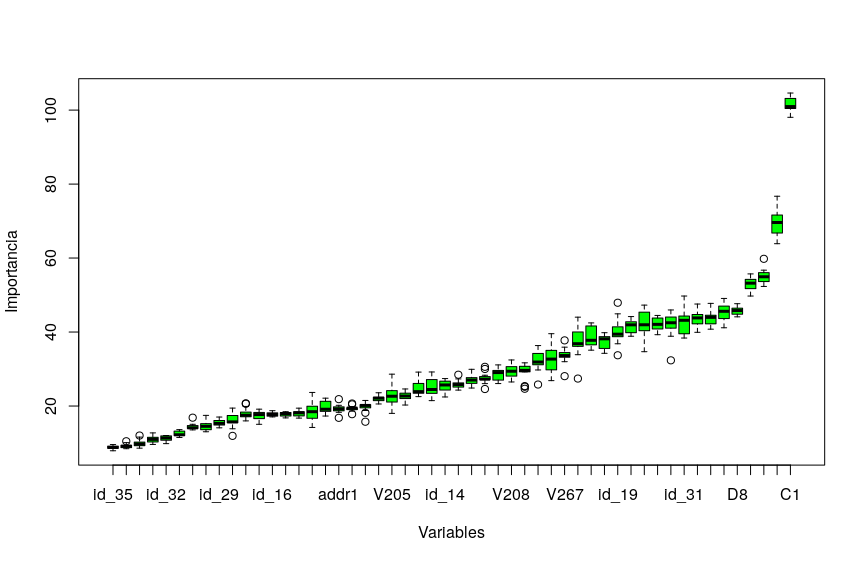
\includegraphics[width=\textwidth]{images/preprocessing/boruta-boxplot.png}
    \caption{Importancia de cada variable calculada por \textit{Boruta}.}
    \label{fig:boruta-boxplot}
\end{figure}

\begin{figure}
    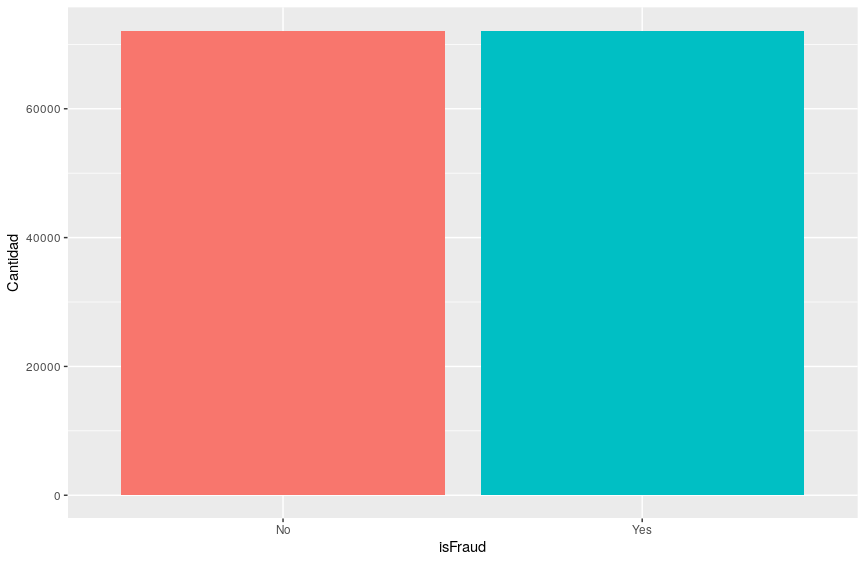
\includegraphics[width=\textwidth]{images/preprocessing/class-rose-barplot.png}
    \caption{Cantidad de ejemplos de cada valor de la clase objetivo presentes en el conjunto de datos balanceado con ROSE.}
    \label{fig:class-rose-barplot}
\end{figure}

\begin{figure}
    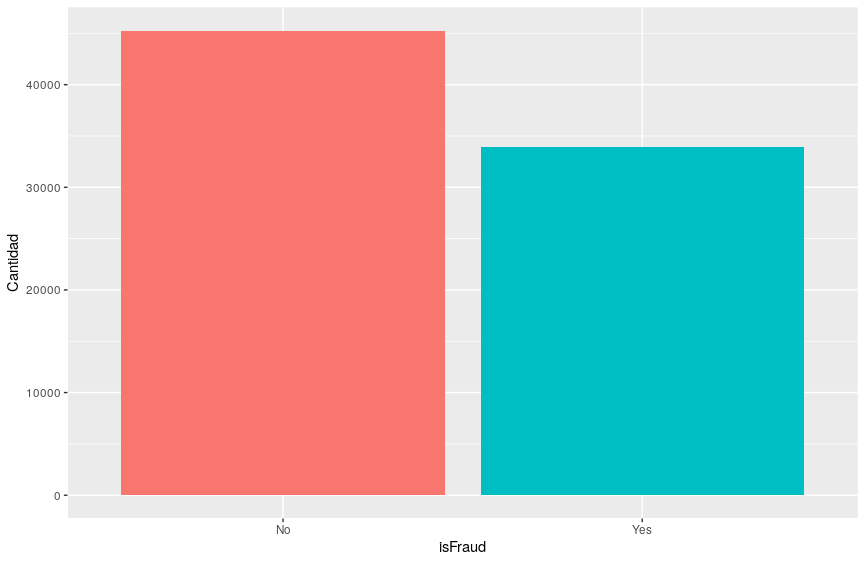
\includegraphics[width=\textwidth]{images/preprocessing/class-smote-barplot.png}
    \caption{Cantidad de ejemplos de cada valor de la clase objetivo presentes en el conjunto de datos balanceado con SMOTE.}
    \label{fig:class-smote-barplot}
\end{figure}
